\documentclass{article}
\usepackage{graphicx} % Required for inserting images





\documentclass[a4paper,12pt]{article}
\usepackage[utf8]{inputenc}
\usepackage{graphicx}
%  Русский язык
\usepackage{multirow}
\usepackage{wrapfig}
\usepackage[T2A]{fontenc}			% кодировка
\usepackage[utf8]{inputenc}			% кодировка исходного текста
\usepackage[english,russian]{babel}	% локализация и переносы

\usepackage{indentfirst} %Красная строка
\usepackage[a4paper,top=1.3cm,bottom=2cm,left=1.5cm,right=1.5cm,marginparwidth=0.5cm]{geometry}
\usepackage[usenames]{color}
\usepackage{colortbl}
\usepackage{csvsimple}
\usepackage{siunitx}
\usepackage{graphicx}
\graphicspath{ {images/} }
\usepackage{tikz}
\usepackage{pgfplots}

\usepackage{amsmath}
\usepackage{floatflt}
\usepackage[left=20mm, top=20mm, right=20mm, bottom=20mm, footskip=10mm]{geometry}

\usepackage{multicol}
\setlength{\columnsep}{2cm}

\usepackage{multicol}
\setlength{\columnsep}{2cm}
\usepackage{hyperref}


% Заметки
\usepackage{todonotes}

% Математика
\usepackage{amsmath,amsfonts,amssymb,amsthm,mathtools} 
\usepackage{hyperref}

\renewcommand{\AA}{\ensuremath{\mathring{A}}}

\begin{document}
\def\figurename{Рисунок}
\begin{titlepage}
\begin{center}
    {\large МОСКОВСКИЙ ФИЗИКО-ТЕХНИЧЕСКИЙ ИНСТИТУТ (НАЦИОНАЛЬНЫЙ ИССЛЕДОВАТЕЛЬСКИЙ УНИВЕРСИТЕТ)}
\end{center}
\begin{center}
    {\largeФизтех-школа биологической и медицинской физики}
\end{center}

\vspace{1cm}
{\huge
\begin{center}
    {\bf Лабораторная работа по общей физике}\\
    \vspace{0.5cm}
    4.3.1. Изучение дифракции света 
\end{center}
}

\vspace{4cm}
\begin{flushright}
{\LARGE Выполнила студентка группы Б06-103:\\ Фитэль Алена \\}

\end{flushright}
\vspace{9cm}
\begin{center}
    Долгопрудный, 2023 г.
\end{center}
\end{titlepage}
\newpage
\section{Введение}
\textbf{Цель работы}: исследовать явления дифракции Френеля и Фраунгофера на щели, изучить влияние дифракции на разрешающую способность оптических инструментов.


\textbf{В работе используются}: оптическая скамья, ртутная лампа, монохроматор, щели с регулируемой шириной, рамка с вертикальной нитью, двойная щель, микроскоп на поперечных салазках с микрометрическим винтом, зрительная труба.

\section{Теоретические сведения}
\subsection*{А. Дифракция Френеля}
\begin{figure}[h!]
	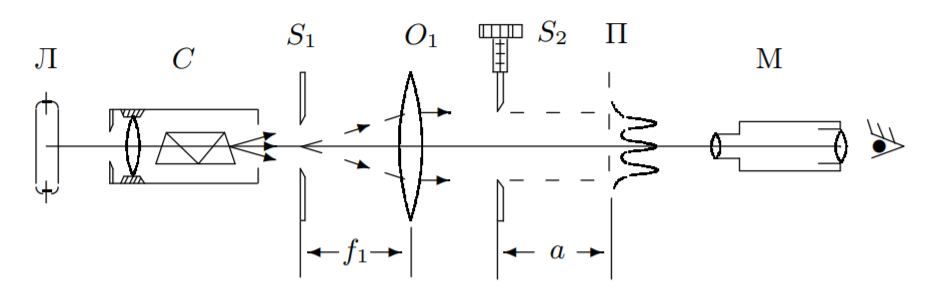
\includegraphics[scale=0.7]{0.png}
	\centering
	\caption{Схема установки 1.}
\end{figure}
При освещении $S_2$ параллельным пучком лучей (плоская зона) зоны Френеля представляют собой плоскости, параллельные краям щели. Результирующая амплитуда в точке наблюдения определеяется суперпозицией колебаний от тех зон Френеля, которые не перекрыты створками щели. Графическое определение результирующей амплитуды производится с помощью векторной диаграммы -- спирали Корню. Суммарная ширина $m$ зон Френеля $z_m$ определяется соотношением:
\begin{equation}
z_m = \sqrt{am\lambda},
\end{equation}
где $a$ -- расстояние от щели до плоскости П. 
\subsection*{Б. Дифракция Фраунгофера на щели}

Дифракцию Фраунгофера можно наблюдать на установке Рис. 1, но для удобства к подобной установке добавляется объектив $O_2$.

\begin{figure}[h!]
	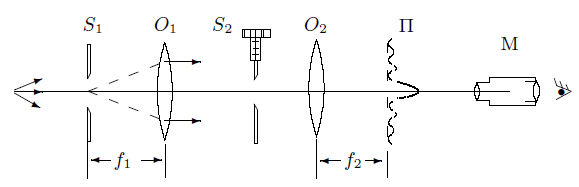
\includegraphics[width = 0.7\textwidth]{3.png}
	\centering
	\caption{Схема установки 2.}
\end{figure}
Дифракционная картина здесь наблюдается в фокальной плоскости объектива $O_2$. Каждому значению $\theta$ соответствует в этой плоскости точка, отстоящая от оптической оси на расстоянии 
\begin{equation}
X = f_2 \tan \theta \approx f_2 \theta.
\end{equation}
При $\theta = 0$ разность хода между лучами нулевая, поэтому в центре поля зрения дифракционный максимум. Первый минимум соответствует $\theta_1$ такому, что в точке наблюдения разность хода пробегаем все значения от 0 до $2\pi$. Аналогично рассуждая, для $m$-й полосы
\begin{equation}
\theta_m = \frac{m \lambda}{D}
\end{equation}
Расстояние $X_m$ тёмной полосы от оптической оси из (2) и (3)
\begin{equation}
X_m = f_2m\frac{\lambda}{D}
\end{equation}
\subsection*{В. Дифракция Фраунгофера для двух щелей}
Для наблюдения дифракции Фраунгофера на двух щелях $S_2$ заменим экраном Э с двумя щелями. При этом для оценки влияния ширины входной щели на чёткость вместо $S_1$ поставим щель с микрометрическим винтом.
\begin{figure}[h!]
	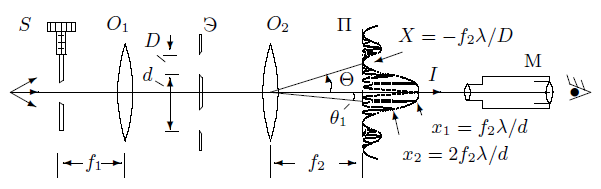
\includegraphics[width = 0.7\textwidth]{4.png}
	\centering
	\caption{Схема установки 3.}
\end{figure}
Два дифракционных изображения входной щели, одно из которых образовано лучами, прошедшими через левую, а другое -- через правую щели, накладываются друг на друга.
Светлая интерфереционная полоса наблюдается в случаях, когда разность хода равна целому числу длин волн. Таким образом, угловая координата максимума порядка $m$ равна
\begin{equation}
\theta_m = \dfrac{m \lambda}{d},
\end{equation}
где $d$ -- расстояние между щелями. Отсюда расстояние между соседними интерфереционными полосами в плоскости П равно
\begin{equation}
\delta x = f_2 \dfrac{\lambda}{d}
\end{equation}
Число интерференционных полос укладывающихся в области центрального максимума равна отношению ширины главного максимума $\frac{2\lambda f_2}{D}$ к расстоянию между соседними полосами:
\begin{equation}
n = \dfrac{2\lambda f_2}{D} \dfrac{1}{\delta f}= \dfrac{2d}{D}.
\end{equation}
При дифракции света на двух щелях чёткая система интерференционных полос наблюдается только при достаточно узкой ширине входной щели $S$. При увеличении ширины картинка пропадает и появляется вновь, но полосы при этом сильно размыты и видны плохо.
\subsection*{Г. Влияние дифракции на разрешающую способность оптического инструмента}
\begin{figure}[h!]
	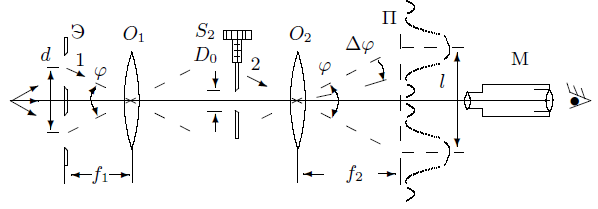
\includegraphics[width = 0.8\textwidth]{5.png}
	\centering
	\caption{Схема установки 4.}
\end{figure}
В отсутствие щели $S_2$ линзы $O_1$ и $O_2$ создают на плоскости П изоюражение щели $S_1$ и это изображение рассматриваются микроскопом М. Таким образом, установку можно рассматривать как оптический инструмент, предназначенные для получения изображения предмета. Если перед $O_2$ расположить $S_2$, то изображение объекта будет искажено из-за дифракции. Чем меньше ширина щели, тем сильнее искажение. Качественной характеристикой этого искажения может служить $\varphi_{min}$ --- минимальное угловое расстояние между объектами (источниками), которые всё ещё воспринимаются как раздельные. Поместим вместо $S_1$ экран Э с двумя щелями с расстоянием $d$. Тогда на $S_2$ будут падать два пучка света с углом
\begin{equation}
\varphi = \dfrac{d}{f_1}
\end{equation}
Из геометрии расстояние $l$ между изображениями щелей в плоскости П равно 
\begin{equation}
l = \varphi f_2 = d \dfrac{f_2}{f_1}.
\end{equation}
Ширина $\Delta \varphi$ определяется дифракцией на $S_2$. Условия, при которых изображения различимы разные для разных наблюдателей, поэтому используют \textit{критерий Рэлея} -- \textit{максимум одного дифракционного пятна должен совпадать с минимумом другого}. В наших условиях это значит, что угловая полуширина $\frac{\lambda}{D}$ равна угловому расстоянию $\frac{l}{f_2}$.
\section{Обработка результатов}
\subsection{Дифракция Френеля на щели}
	Длина волны для этой работы $\lambda = 578$ нм.
\begin{enumerate}
\item Запишем ширину щели $S_2$, измеренную с помощью микрометрического винта щели ($b_1$) и шкалы микроскопа ($b_2$):
	\[
		b_1 = 0,40\pm0,02 \text{ мм}
	\]
	\[
		b_2 = 0,38\pm0,01 \text{ мм}
	\]
	
	
\item Добившись наибольшей чёткости дифракционной картины, найдем резкое изображение щели (чёткие края без дифракционных полос). Начальное положение микроскопа --- координата по шкале линейки $x_0 = 35.9\pm0,1 \text{ см}$, расположенной на оптической скамье. 
\item Приближая микроскоп к щели, cнимем зависимость количества темных полос на экране от расстояния микроскопа до плоскости наблюдения. Зависимость количества полос от расстояния до плоскости наблюдения представлена в Таблице 1. Здесь $a_m$ -- смещение от положения $x_0$, $z_m$ находится из формулы (1).

\begin{table}[h!]
{\begin{tabular}{|l|l|r|r|r|r|}
\hline
\textbf{$n$} & \textbf{$m$} & \multicolumn{1}{l|}{\textbf{$x_m$, см}} & \multicolumn{1}{l|}{\textbf{$a_m$, мм}} & \multicolumn{1}{l|}{\textbf{$2z_m$, мкм}} & \multicolumn{1}{l|}{\textbf{$\sigma_{2z_m}$, мкм}} \\ \hline
1 & 2 & 39,2 & 33 & 391 & 8 \\ \hline
2 & 3 & 38,8 & 29 & 448 & 11 \\ \hline
3 & 4 & 38 & 21 & 441 & 15 \\ \hline
4 & 5 & 37,7 & 18 & 456 & 18 \\ \hline
5 & 6 & 37,5 & 16 & 471 & 21 \\ \hline
6 & 7 & 37,3 & 14 & 476 & 24 \\ \hline
\end{tabular}%
}
\centering
\caption{Зависимость $z_m = f(a_m)$.}
\end{table}\\

\item Построим график зависимости величины $ 2\xi_n $  от $ n $. Поскольку суммарная ширина зон Френеля не меняется и равна $D$, график должен представлять горизонтальную прямую. Аппроксимируем полученную зависимость горизонтальной прямой методом хи-квадрата. Полученная таким образом ширина щели - $D = 460\pm 70$ мкм. Видно, что ширина френелевских зон - величина порядка ширины щели. 

 \begin{figure}[h!]
    \centering
    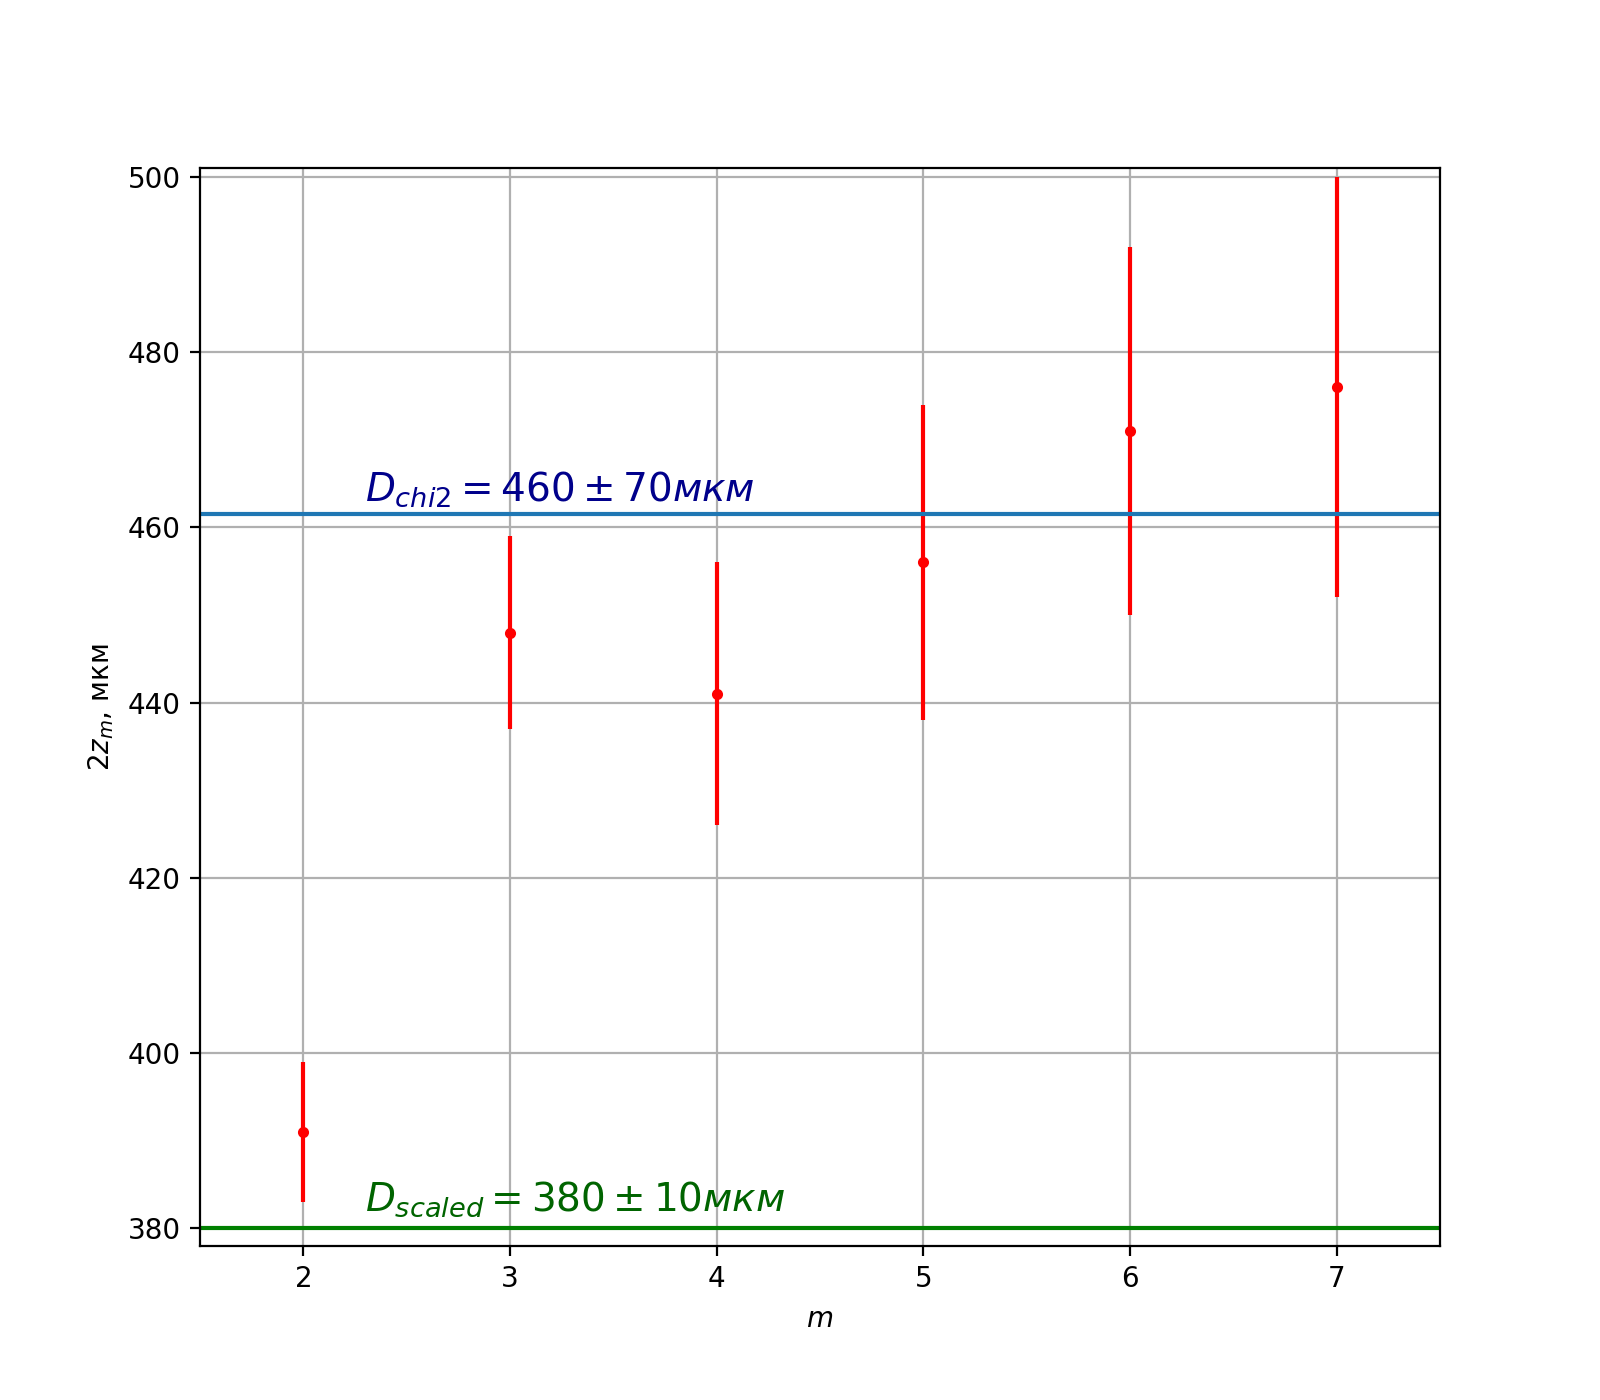
\includegraphics[width=12cm]{4.3.1(1).png}
    \caption{График зависимости сумманой толщины зон Френеля от их числа.}
    \label{fig:vac}
\end{figure}

\item Для исследования дифракции Френеля на препятствии поставим вместо щели~$S_2$ рамку с тонкой вертикальной нитью. Настроим микроскоп на резкое изображение нити. При удалении микроскопа от нити на её фоне всегда наблюдается чётное число тёмных дифракционных полос (светлый центр).
\end{enumerate}
\newpage	
\subsection{Дифракция Фраунгофера на щели}
 Фокусное расстояние линз $f_{O_1} = 10{,}8$ см, $f_{O_2} = 13{,}8$ см. Диаметр щели по показаниям микрометрического винта $D = 370\pm5$ мкм.
 \begin{enumerate}
     \item
Измерим с помощью винта поперечного перемещения микроскопа координаты $ X_m $ нескольких дифракционных минимумов. Результаты занесем в табл. 2 и построим график зависимости минимумов от их номеров. 
 
	\begin{table}[h!]
\centering
{%
\begin{tabular}{|r|r|r|r|}
\hline
\multicolumn{1}{|l|}{\textbf{m}} & \multicolumn{1}{l|}{\textbf{x_{max}, мм}} & \multicolumn{1}{l|}{\cellcolor[HTML]{FFFFFF}\textbf{x_{min}, мм}} & \multicolumn{1}{l|}{\textbf{x, мм}} \\ \hline
-3 & 1,6 & 1,52 & 1,56 \\ \hline
-2 & 1,82 & 1,76 & 1,79 \\ \hline
-1 & 1,98 & 2,02 & 2 \\ \hline
1 & 2,48 & 2,42 & 2,45 \\ \hline
2 & 2,68 & 2,62 & 2,65 \\ \hline
3 & 2,9 & 2,82 & 2,86 \\ \hline
\end{tabular}%
}
\caption{Координаты минимумов дифракции Фраунгофера}
\label{tab:my-table}
\end{table}

\begin{figure}[h!]
    \centering
    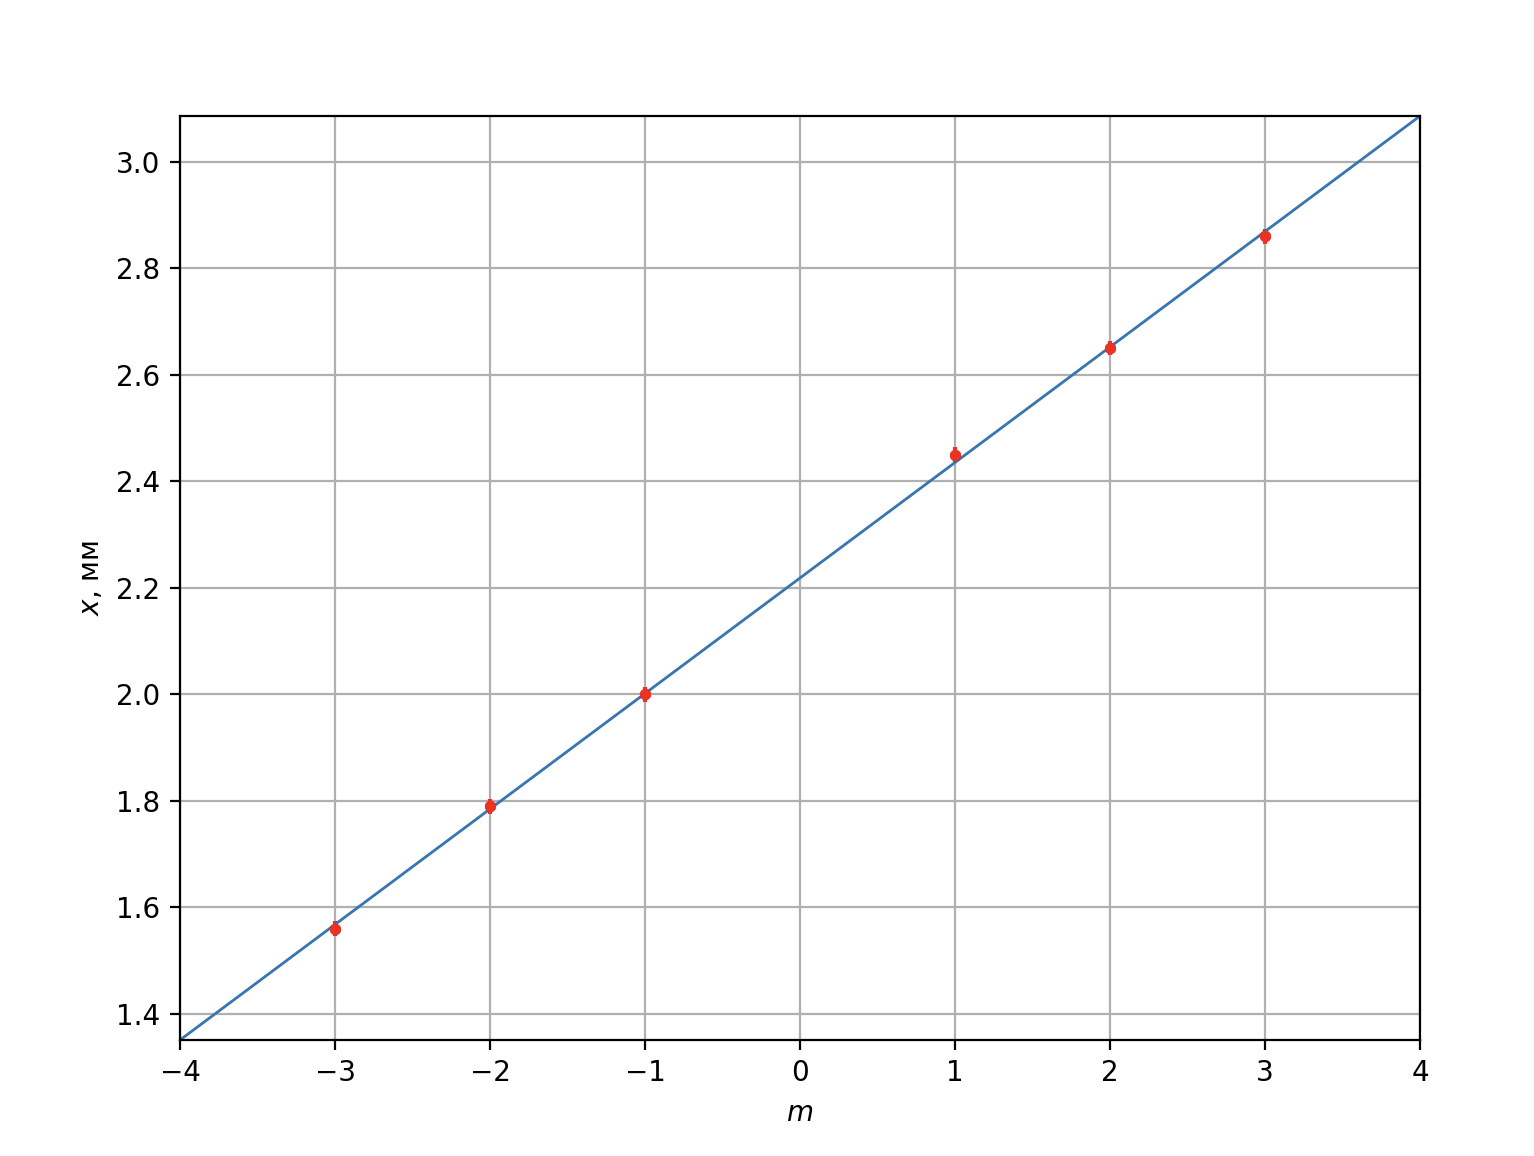
\includegraphics[width=11cm]{4.3.1(2).png}
    \caption{График зависимости $X_m = f(m)$.}
    \label{fig:vac}
\end{figure}


	\item По наклону графика методом наименьших квадратов определим среднее расстояние между соседними минимумами: $\Delta X = 217 \pm 2$ мкм. Пользуясь этим результатом, с помощью формулы (4) получим значение $D$:
	\begin{equation*}
	D = \dfrac{f_2m\lambda}{X_m} = \dfrac{f_2 \lambda}{\Delta X} = 368\pm3\text{ мкм}.
	\end{equation*}
\end{enumerate}
 \newpage
\subsection{Дифракция Фраунгофера на двух щелях}
Получим дифракционную картину от двух щелей. Ширина центрального максимума при $ b=0.055\pm 0.001\; мм $ равна
\begin{equation*}\label{key}
	X = 1.10\pm 0.03 \text{ мм}
\end{equation*}
и он включает в себя $ n = 13 $ светлых промежутков.
Первое исчезновение интерференционных полос при
\begin{equation*}\label{key}
	b_0 = 0.40 \pm 0.01 \text{ мм}.
\end{equation*}
Расстояние между минимумами равно:
\begin{equation*}\label{key}
	\delta x \approx \frac{X}{n} = 0.085\pm 0.006 \text{ мм}
\end{equation*}
Из формулы (6):
\begin{equation*}\label{key}
	d = \frac{\lambda f_2}{\delta x} = 0.94\pm 0.07 \text{ мм}.
\end{equation*}
Это значение отличается от замеренного: фактическое расстояние между щелями $ d_{measured} = 0.70\pm 0.02\text{ мм} $. 
\subsection{Влияние дифракции на разрешающую способность}
	
	Запишем максимальную ширину щели $b_{measured} = 0,092\pm 0,001$ мм, при которой еще различимо изображение щели.
	
	Для проверки справедливости критерия Релея рассчитаем эту величину по формуле
	\[
		b_0 = \frac{\lambda}{d}F_1 = 0,089\pm 0,003 \text{ мм}
	\]
	\section{Обсуждение результатов и вывод}

 В ходе работы было изучено явление дифракции света - дифракция Френеля на щели и на препятствии, дифракция Фраунгофера на одной и двух щелях, влияние дифракции на разрешающую способность оптических приборов.

\begin{itemize}
    \item При исследовании явления дифракции Френеля на щели было полученно, что ширина зон Френеля совпадает по порядку величины с действительной шириной щели, измеренной микрометрическим винтом. 

\item При дифракции на препятствии при удалении микроскопа от нити на её фоне всегда наблюдали чётное число тёмных дифракционных полос и светлый центр.

    \item Значение для ширины щели, вычисленное по формуле (4), совпадает в пределах погрешности с величиной, измеренной по микрометрической шкалой:
 \begin{center}
        $D_{measured} = 370\pm5$ мкм \hspace{1cm} $D = 368\pm3$ мкм
    \end{center}
Это подтверждает теоретические выкладки и говорит о выполнении предложенной теории.
    
    \item При исследовании явления дифракции Фраунгофера на двух щелях было получено значение расстояния между щелями, совпадающее в пределах погрешости $2\delta$ с измеренным по микрометрической шкале:
     
    \begin{center}
        $d = 0.94\pm 0.07 \text{ мм} $ \hspace{1cm} $ d_{measured} = 0.70\pm 0.02\text{ мм} $
    \end{center}

\item В ходе работы была произведена оценка влияния дифракции на разрешающую способность оптического прибора. В результате измерений получаем, что $b_0 < b_{measured}$.

\end{itemize}



\end{document}
